\documentclass[a4paper]{article}

\usepackage{pdp}

%------------------------------------------------------------------------------
%	REPORT INFORMATION
%------------------------------------------------------------------------------

\title{ProjectName -- C/Java/Python}
\subtitle{Rapport préliminaire}
\author{Étudiant1, Étudiant2, Étudiant3, Étudiant4, Étudiant5}

%------------------------------------------------------------------------------

\begin{document}

%------------------------------------------------------------------------------
%	TITLE PAGE
%------------------------------------------------------------------------------

\maketitle
\thispagestyle{empty}

%------------------------------------------------------------------------------
%	MAIN MATTER
%------------------------------------------------------------------------------

\section*{Introduction}

Lorem ipsum dolor sit amet, consectetur adipiscing elit. Sed do eiusmod tempor
incididunt ut labore et dolore magna aliqua. Ut enim ad minim veniam, quis
nostrud exercitation ullamco laboris nisi ut aliquip ex ea commodo consequat.
Duis aute irure dolor in reprehenderit in voluptate velit esse cillum dolore eu
fugiat nulla pariatur. Excepteur sint occaecat cupidatat non proident, sunt in
culpa qui officia deserunt mollit anim id est laborum.

Pellentesque iaculis molestie euismod. In hac habitasse platea dictumst. Duis eu
gravida sem. Vivamus pulvinar, tellus auctor sollicitudin iaculis, quam massa
blandit ligula, in mollis est tellus et velit. Nulla gravida sapien nibh, nec
faucibus lorem aliquam sed. Curabitur rutrum elit purus, et congue neque
venenatis vitae. Sed non magna nisi. Pellentesque euismod non ipsum a hendrerit.
Pellentesque vehicula tincidunt lacinia. Sed rhoncus porttitor facilisis.

Etiam sed molestie odio. Nunc cursus sollicitudin est vitae posuere. Nullam
pellentesque metus eu dui porttitor bibendum. Morbi egestas arcu ut urna dictum
placerat non non nisl. Quisque non ante in eros cursus pulvinar. Sed augue
libero, eleifend a urna eget, pellentesque condimentum odio. Sed sed dui non
diam mattis interdum eget sed urna. Integer consectetur, erat id rutrum posuere,
dui velit dictum mi, quis tincidunt magna diam sit amet nunc. Etiam dui augue,
sollicitudin rhoncus nisl a, rhoncus tempor purus.

Suspendisse cursus erat et metus fermentum ullamcorper. Etiam eros arcu, dapibus
quis efficitur ut, congue id nunc. Pellentesque aliquam venenatis convallis.
Nulla nisi justo, aliquet quis lacus eget, aliquet maximus velit. Maecenas ex
turpis, iaculis eget dignissim non, efficitur vel mi. Maecenas pharetra elit
ornare sem suscipit ornare id id sapien. Vivamus sem neque, consectetur vitae
aliquet non, finibus eu lectus. Fusce aliquam ipsum ut viverra vehicula. Donec
ultrices varius nulla vel finibus. Donec convallis fringilla ante id porta.

\section{Première section}

Lorem ipsum dolor sit amet, consectetur adipiscing elit. Sed do eiusmod tempor
incididunt ut labore et dolore magna aliqua. Ut enim ad minim veniam, quis
nostrud exercitation ullamco laboris nisi ut aliquip ex ea commodo consequat.
Duis aute irure dolor in reprehenderit in voluptate velit esse cillum dolore eu
fugiat nulla pariatur. Excepteur sint occaecat cupidatat non proident, sunt in
culpa qui officia deserunt mollit anim id est laborum.

\section{Algorithmes et Structures de Données}

L'implémentation d'un joueur artificiel performant au Scrabble repose sur la résolution de deux problèmes distincts : la génération efficace de tous les coups légaux et la sélection du meilleur coup parmi ceux-ci. Cette section détaille les choix algorithmiques retenus pour répondre à ces besoins.

\subsection{Modélisation du problème}

Contrairement aux Échecs ou au Go, qui sont des jeux à information parfaite et déterministes, le Scrabble est un jeu à information imparfaite, on ne connait pas lettres de l'adversaire et le tirage des lettres repose sur le hasard.

Une approche gloutonne, qui consisterait à jouer systématiquement le coup rapportant le plus de points à l'instant $t$, est sous-optimale. Elle néglige deux facteurs cruciaux :
\begin{itemize}
    \item \textbf{Le reliquat (Rack Leave) :} La qualité des lettres conservées pour le tour suivant.
    \item \textbf{L'ouverture du plateau :} Le risque d'offrir une case "Mot Compte Triple" à l'adversaire.
\end{itemize}

Pour pallier ces manques, nous avons deux algorithmes de théorie des jeux : Minimax et Expectiminimax.

\subsection{L'Algorithme Minimax}

L'algorithme Minimax est la base de la décision dans les jeux à somme nulle. Il parcourt l'arbre de jeu jusqu'à une profondeur $d$ donnée.

\subsubsection*{Fonctionnement}
L'algorithme alterne entre deux types de nœuds :
\begin{itemize}
    \item \textbf{Nœuds MAX :} Cherche à maximiser le score final.
    \item \textbf{Nœuds MIN :} Cherche à minimiser le score.
\end{itemize}

L'application stricte de Minimax au Scrabble pose un problème de modélisation. Minimax suppose que l'adversaire jouera toujours le coup optimal pour nous contrer. Or, pour déterminer ce coup optimal, l'algorithme doit connaître les lettres de l'adversaire.
Dans une simulation Minimax, nous devrions supposons le pire cas: l'adversaire possède exactement les lettres nécessaires pour réfuter notre coup (ex: un "Z" pour atteindre un mot compte triple ouvert). Cette approche rend l'IA excessivement défensive et inadaptée à la réalité probabiliste du tirage.

\subsection{L'Algorithme Expectiminimax}

Pour intégrer la dimension aléatoire du tirage de lettres, nous utilisons l'algorithme \textbf{Expectiminimax}. C'est une variation du Minimax qui introduit un troisième type de nœud : les \textbf{Nœuds de Hasard}.

L'arbre de décision se décompose désormais en trois niveaux par tour de jeu :
\begin{enumerate}
    \item \textbf{Nœud MAX :} L'IA choisit un coup parmi les coups possibles générés.
    \item \textbf{Nœud CHANCE :} Ce nœud représente l'incertitude sur les lettres de l'adversaire. Il possède une branche pour chaque tirage possible, pondérée par sa probabilité.
    \item \textbf{Nœud MIN :} L'adversaire joue le meilleur coup possible avec le tirage attribué par le nœud chance.
\end{enumerate}

La valeur d'un nœud de hasard n'est ni un minimum ni un maximum, mais une espérance mathématique. Pour un état $s$ correspondant à un nœud de hasard :

\[
\text{Expect}(s) = \sum_{r \in \text{Tirages}} P(r) \times v(\text{successeur}(s, r))
\]

Où $P(r)$ est la probabilité que le tirage soit $r$, sachant les lettres déjà visibles.

\subsubsection*{Défi combinatoire et Échantillonnage}
Le facteur de branchement aux nœuds de hasard est gigantesque. Simuler tous les tirages possibles de 7 lettres parmi les $N$ lettres restantes est impossible en temps réel.

Pour contourner cette complexité, nous utiliserons une méthode d'approximation par échantillonnage. Au lieu de calculer la somme sur tous les tirages, nous générons un sous-ensemble représentatif de $N$ mains adverses aléatoires (ex: 20 simulations) basées sur la distribution réelle des lettres restantes.

L'algorithme devient alors :
\begin{enumerate}
    \item L'IA joue un coup $C$.
    \item Nous simulons $N$ mains adverses possibles.
    \item Pour chaque main, nous calculons la meilleure réponse de l'adversaire.
    \item La valeur du coup $C$ est la moyenne des scores résultant de ces simulations.
\end{enumerate}

{\large
  \begin{minted}[frame=single]{python}
def hello_world():
    print("Hello, World!")
hello_world()
  \end{minted}
}

Un exemple d'image flottante (Fig.~\ref{fig:example}).

\begin{figure}[!ht]
  \centering
  \frame{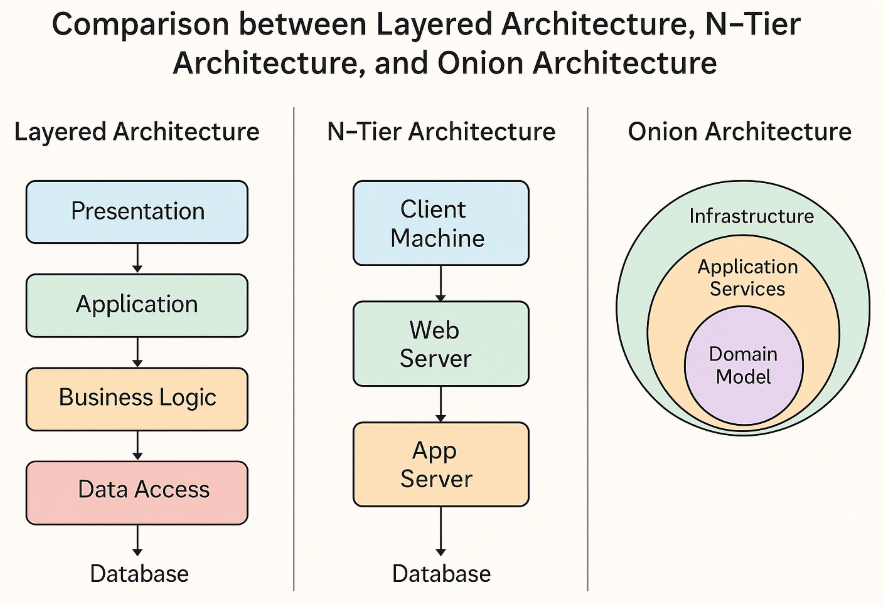
\includegraphics[width=.85\textwidth]{layered_architectures.png}}
  \caption{Une architecture en couches}\label{fig:example}
\end{figure}

\section*{Conclusion}

Suspendisse sit amet nisi placerat, vestibulum nisl vel, iaculis nunc.
Suspendisse quis libero vel ipsum gravida congue nec id arcu. Donec vel mi
viverra, commodo urna vitae, tincidunt lectus. Fusce pellentesque, lectus a
placerat vestibulum, magna lectus placerat nibh, vehicula pellentesque lacus
erat non nulla. Suspendisse maximus, turpis at suscipit egestas, libero massa
ultrices libero, at tincidunt velit eros a eros. Maecenas id tempor nunc.
Phasellus condimentum porttitor sapien in sagittis. Proin in metus diam. Mauris
in turpis sed ex viverra iaculis. Sed lobortis, tellus vitae congue blandit, leo
elit auctor libero, id tempor ante dolor quis quam. Donec eget ligula quam.
Maecenas porttitor massa vel felis elementum tristique.

%------------------------------------------------------------------------------
%	BIBLIOGRAPHY
%------------------------------------------------------------------------------

\nocite{*}
\bibliographystyle{plain}
\bibliography{bibliography}

%------------------------------------------------------------------------------
% BACK MATTER
%------------------------------------------------------------------------------
\appendix

\section{Section en annexe}

Lorem ipsum dolor sit amet, consectetur adipiscing elit. Sed do eiusmod tempor
incididunt ut labore et dolore magna aliqua. Ut enim ad minim veniam, quis
nostrud exercitation ullamco laboris nisi ut aliquip ex ea commodo consequat.
Duis aute irure dolor in reprehenderit in voluptate velit esse cillum dolore eu
fugiat nulla pariatur. Excepteur sint occaecat cupidatat non proident, sunt in
culpa qui officia deserunt mollit anim id est laborum.

\end{document}
